\chapter{Diseño e implementación} % Main chapter title
\label{Chapter3} % Change X to a consecutive number; for referencing this chapter elsewhere, use \ref{ChapterX}
En este capitulo se detalla el HW desarrollado en etapas con un enfoque individual a cada etapa. Se presentan circuitos esquematicos correspondientes al circuito implementado para cada etapa individual y su rol en el sistema. 
La subseccion \ref{seccion_firmware} expone el patron \textit{power save loop} adoptado en la logica de negocios, los perifericos del MC con los cuales interactua y la rutina de interrupcion que atiende al generarse un corte.
Por ultimo, la seccion \ref{seccion_bes} da al lector detalle acerca de la integracion entre la red LoRaWAN y los servicios adoptados para este proyecto.

\definecolor{mygreen}{rgb}{0,0.6,0}
\definecolor{mygray}{rgb}{0.5,0.5,0.5}
\definecolor{mymauve}{rgb}{0.58,0,0.82}

%%%%%%%%%%%%%%%%%%%%%%%%%%%%%%%%%%%%%%%%%%%%%%%%%%%%%%%%%%%%%%%%%%%%%%%%%%%%%
% parámetros para configurar el formato del código en los entornos lstlisting
%%%%%%%%%%%%%%%%%%%%%%%%%%%%%%%%%%%%%%%%%%%%%%%%%%%%%%%%%%%%%%%%%%%%%%%%%%%%%
\lstset{ %
  backgroundcolor=\color{white},   % choose the background color; you must add \usepackage{color} or \usepackage{xcolor}
  basicstyle=\footnotesize,        % the size of the fonts that are used for the code
  breakatwhitespace=false,         % sets if automatic breaks should only happen at whitespace
  breaklines=true,                 % sets automatic line breaking
  captionpos=b,                    % sets the caption-position to bottom
  commentstyle=\color{mygreen},    % comment style
  deletekeywords={...},            % if you want to delete keywords from the given language
  %escapeinside={\%*}{*)},          % if you want to add LaTeX within your code
  %extendedchars=true,              % lets you use non-ASCII characters; for 8-bits encodings only, does not work with UTF-8
  %frame=single,	                % adds a frame around the code
  keepspaces=true,                 % keeps spaces in text, useful for keeping indentation of code (possibly needs columns=flexible)
  keywordstyle=\color{blue},       % keyword style
  language=[ANSI]C,                % the language of the code
  %otherkeywords={*,...},           % if you want to add more keywords to the set
  numbers=left,                    % where to put the line-numbers; possible values are (none, left, right)
  numbersep=5pt,                   % how far the line-numbers are from the code
  numberstyle=\tiny\color{mygray}, % the style that is used for the line-numbers
  rulecolor=\color{black},         % if not set, the frame-color may be changed on line-breaks within not-black text (e.g. comments (green here))
  showspaces=false,                % show spaces everywhere adding particular underscores; it overrides 'showstringspaces'
  showstringspaces=false,          % underline spaces within strings only
  showtabs=false,                  % show tabs within strings adding particular underscores
  stepnumber=1,                    % the step between two line-numbers. If it's 1, each line will be numbered
  stringstyle=\color{mymauve},     % string literal style
  tabsize=2,	                   % sets default tabsize to 2 spaces
  title=\lstname,                  % show the filename of files included with \lstinputlisting; also try caption instead of title
  morecomment=[s]{/*}{*/}
}


%----------------------------------------------------------------------------------------
%	SECTION 1
%----------------------------------------------------------------------------------------
\section{Detalle del hardware por etapas}
\subsection{Circuito de selección de modo}
Considerando el caso límite donde el nivel del acumulador es bajo y el MC ordena al relay (RL) con retención cambiar su estado, la energía necesaria para excitar al RL puede generar una caída de tensión significativa en el acumulador y resultar en un circuito totalmente desenergizado sin posibilidad de volver a entrar en operación a no ser mediante la intervención humana.\\
Un caso extremo como el mencionado, implica que el HW posea un mecanismo para restablecer su operación tras largos periodos de tiempo aun después de haberse vaciado el acumulador.\\
En la figura \ref{fig:ctoselecciondemodo} se implementó el RL sin retención presentado en \ref{fig:relay} y su circuito de mando. Los terminales del TI, se encuentran conectados por defecto a la etapa de conversión y acumulacion de energía (terminales \textit{NC1} y \textit{NC2}). Una vez que la tensión en bornes del acumulador alcanza el valor de mínimo para que el conversor DC/DC entre en operación, también la electrónica sin la necesidad de una intervención externa.\\
% TODO: \usepackage{graphicx} required
\begin{figure}[h]
	\centering
	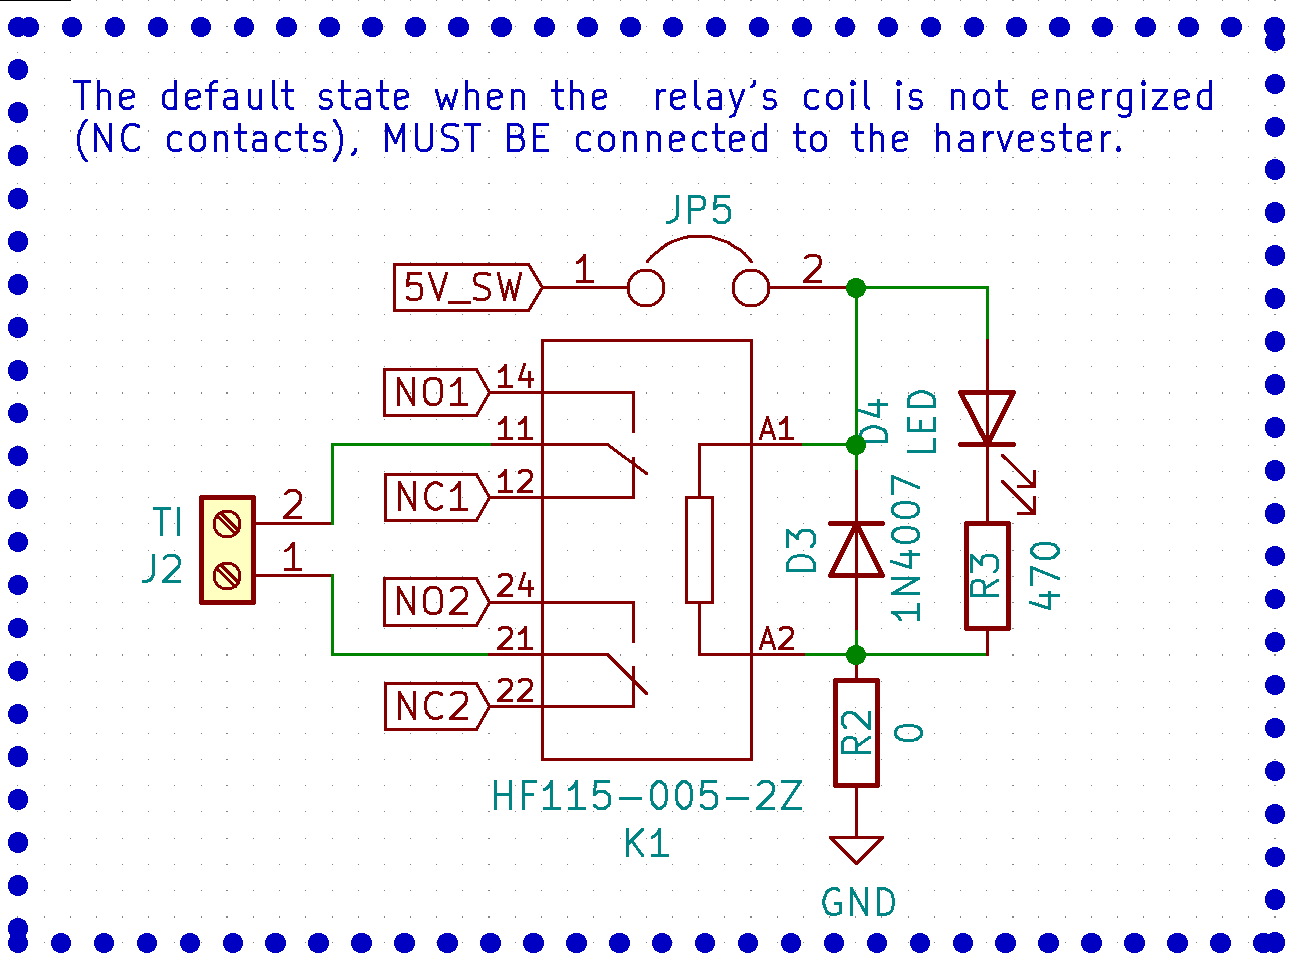
\includegraphics[width=0.7\linewidth]{Figures/cto_seleccion_de_modo}
	\caption{circuito selector de modo basado en el relay HF115-005-2ZS4}
	\label{fig:ctoselecciondemodo}
\end{figure}\\
Cada vez que se desea tomar una medición de corriente, el MC enciende la bobina del relay y conecta el TI al circuito de medición de valor RMS. Al \\

\subsection{Puente rectificador de onda completa}
Para el prototipo desarrollado en este trabajo, se replicó el circuito rectificador de onda completa presentado en la figura \ref{fig:rect_MOSFET}. Con el objeto de reducir el espacio ocupado en el PCB, se optó por utilizar un chip DMHC3025 en encapsulado SOIC-8 [REFERENCIA A DATASHEET]. El encapsulado presentado en la \ref{fig:esquematicointernorctificadormosfet} alberga un puente H formado dos transistores MOSFET tipo P y dos tipo N. Las características eléctricas de relevancia para esta aplicacion son presentadas en la tabla \ref{tabla_transistores_rectificador}.
\begin{table}[h]
	\centering
	\caption{Características eléctricas de los transistores que forman parte del rectificador de onda completa.}
	\begin{tabular}{cc} 
		\hline
		\textbf{\textbf{Parámetro}} & \begin{tabular}[c]{@{}c@{}}\textbf{}\\\textbf{\textbf{Valor máximo}}\end{tabular}  \\ 
		\hline
		Rds                         & 25 miliohms                                                                        \\
		Id                          & 6 A                                                                                \\
		Vdss                        & 30 V                                                                               \\
		\hline
	\end{tabular}\label{tabla_transistores_rectificador}
\end{table}

% TODO: \usepackage{graphicx} required
\begin{figure}[h]
	\centering
	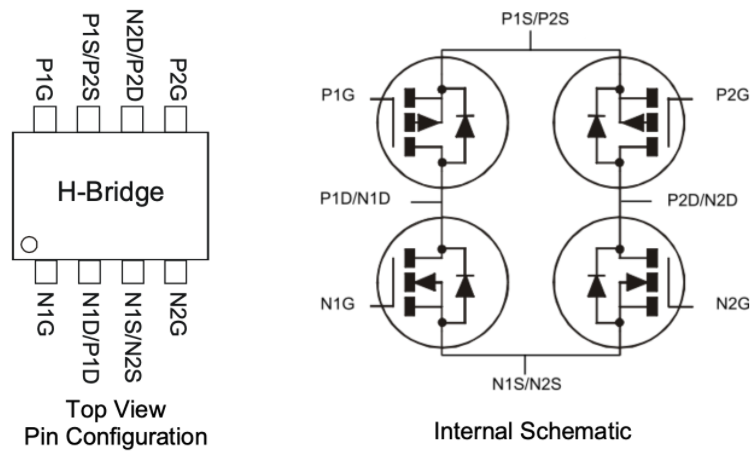
\includegraphics[width=0.8\linewidth]{Figures/esquematico_interno_rctificador_mosfet}
	\caption{Pinout y esquematico interno del DMHC3025 [referencia al datasheet].}
	\label{fig:esquematicointernorctificadormosfet}
\end{figure}
El circuito final implementado encargado de la recitificacion y filtrado de la tension DC a la salida se presenta en la figura \ref{fig:ctorectificacionfiltrado}. Dos diodos zener \textit{D1} y \textit{D2} en antiparalelo protegen el a los transistores  de picos de sobretensión recortando la onda a 27 V para cada semiciclo de la onda senoidal a la entrada.\\
% TODO: \usepackage{graphicx} required
\begin{figure}
	\centering
	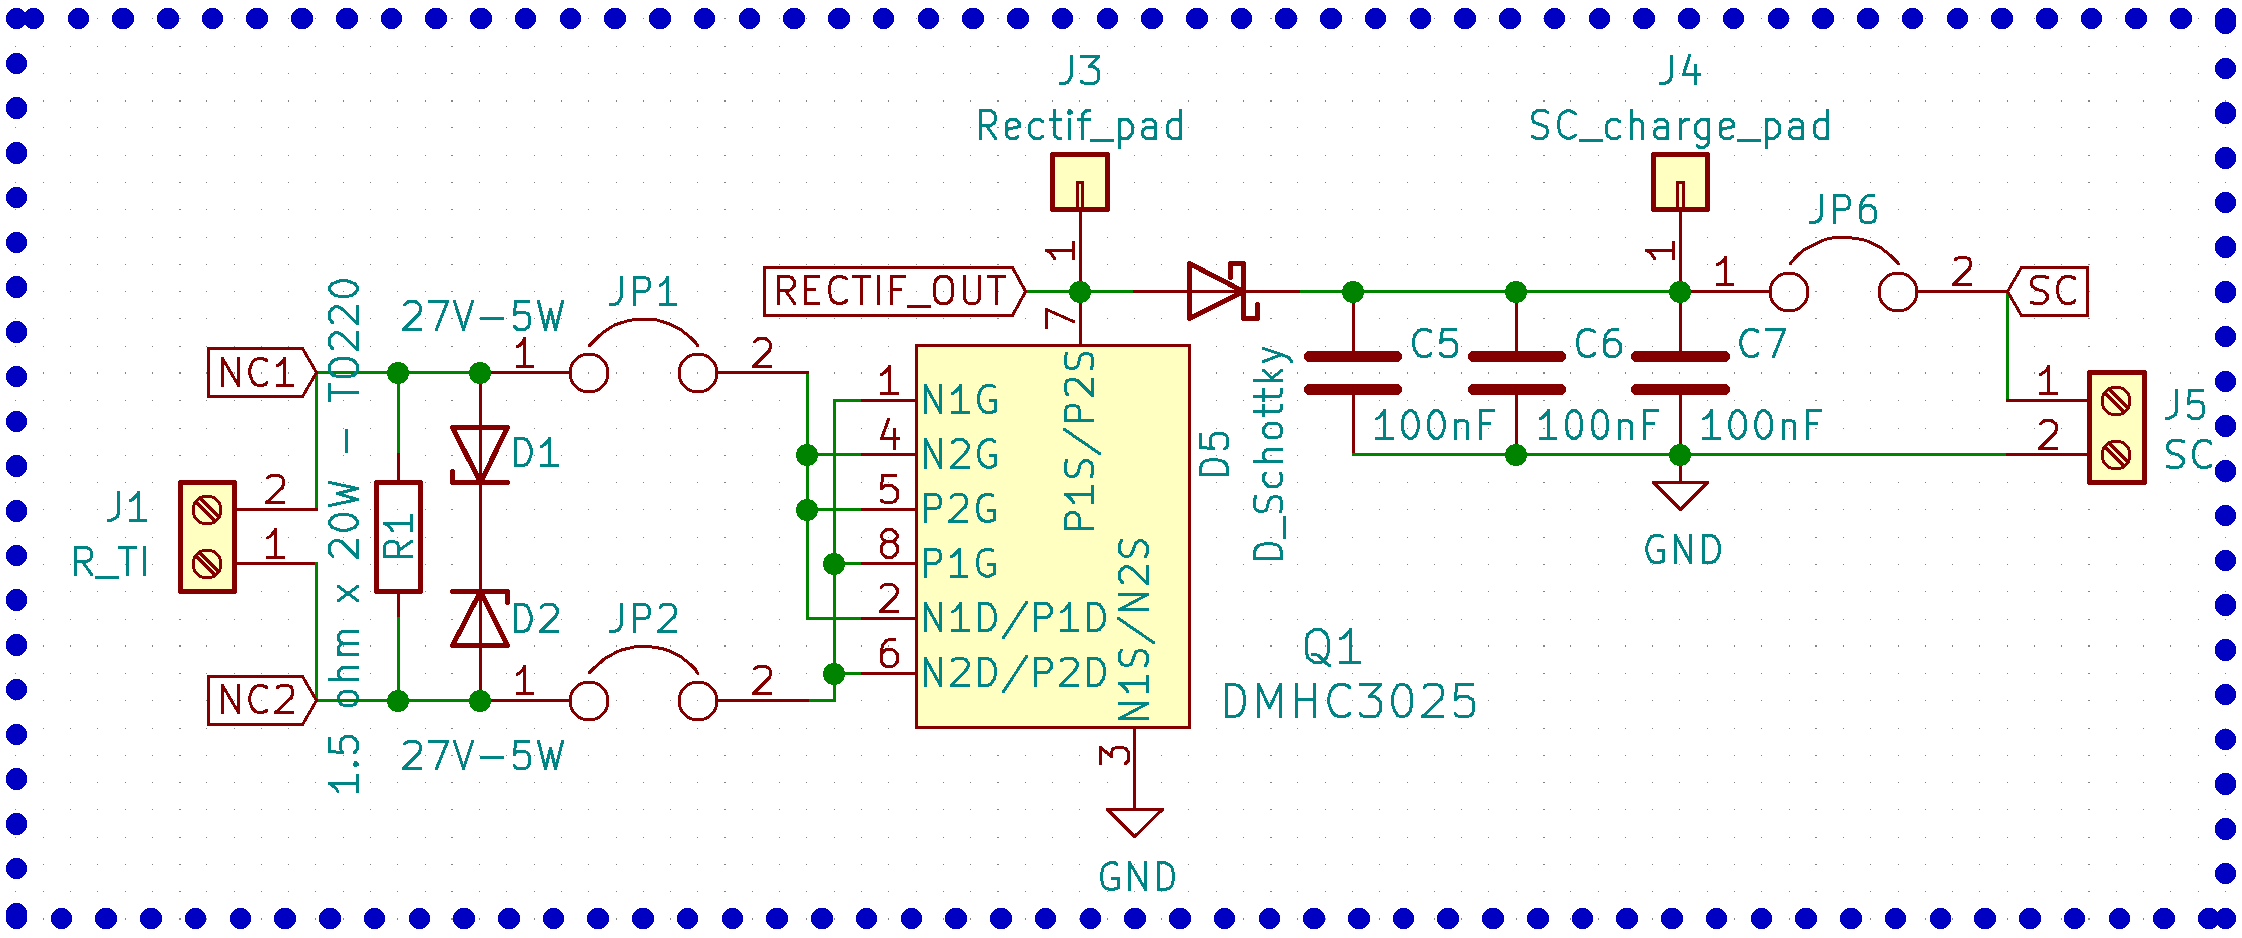
\includegraphics[width=0.8\linewidth]{Figures/cto_rectificacion_filtrado}
	\caption{Etapa de rectificacion, filtrado y acumulacion implementada.}
	\label{fig:ctorectificacionfiltrado}
\end{figure}\\
A su salida, un conjunto de capacitores cerámicos \textit{C5}, \textit{C6} y \textit{C7} filtran ruido de alta frecuencia para luego acumular toda la energía en el SC conectado a \textit{J5}.\\

\subsection{Acumulador de energía basado en supercapacitores}
A la salida del rectificador de onda completa de la figura \ref{fig:ctorectificacionfiltrado}, se conecta en la bornera \textit{J5} un banco de dos SC de 500 F x 2,7 V en serie con una capacitancia equivalente de 250F x 5,4 V.\\
Los SC, se presentan en la figura \ref{fig:imagensupercap} como un módulo único donde ya se encuentran montados sobre una placa con una electrónica adicional de protección. El circuito de protección, se encarga de limitar la tensión en sus bornes a 2,5 V y disipar la potencia excedente.\\
% TODO: \usepackage{graphicx} required
\begin{figure}[h]
	\centering
	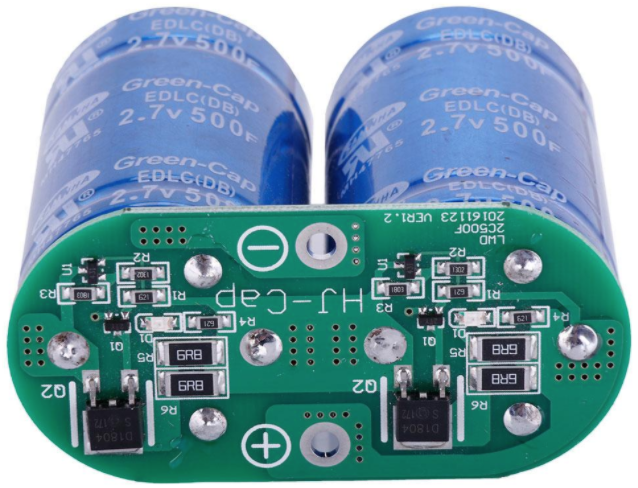
\includegraphics[width=0.7\linewidth]{Figures/imagen_supercap}
	\caption{Banco de SC de 250 F x 5,4 V utilizado como acumulador.}
	\label{fig:imagensupercap}
\end{figure}\\
Al tratarse de una capacitancia total considerablemente mayor que la de un capacitor habitual, almacenará también más energía. El SC puede entonces cumplir la función de acumular energía para mantener operativa la electrónica en caso de que se interrumpa la conversión de energía.\\
Adicionalmente el módulo elegido, aporta simpleza al esquemático final y un rango de temperatura de operación mayor que una solución que además incluya una batería \citep{PORCARELLI20141671}.\\

 \subsection{Circuito de detección de cortes}
 Una de las funcionalidades relevantes del HW, es detectar interrupciones en la distribución de energía debido a razones tales como sobrecarga en la línea o desastres naturales.\\
 El circuito detector de cortes propuesto en Figura detector está basado en un comparador TLV3691 de la firma Texas Instruments. Su salida, se encarga de generar una interrupcion (IRQ) por flanco ascendente y despertar al MC.\\
 % TODO: \usepackage{graphicx} required
 \begin{figure}[h]
 	\centering
 	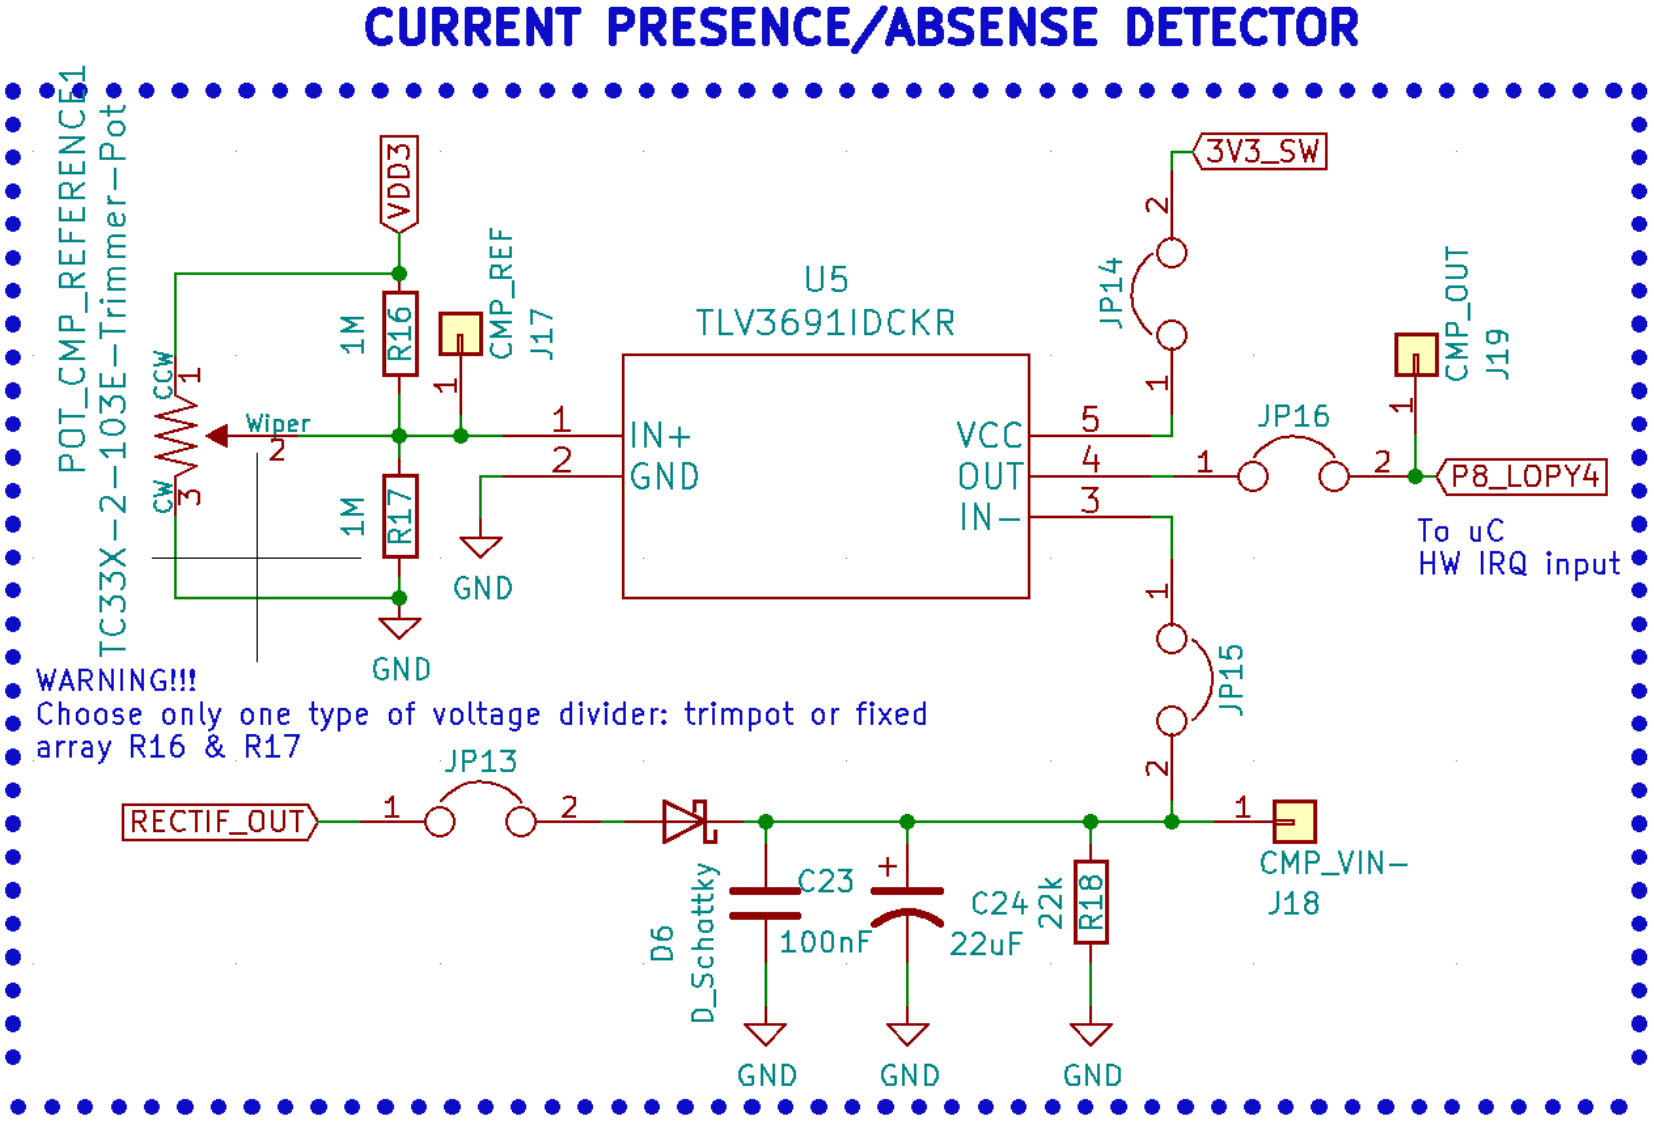
\includegraphics[width=0.7\linewidth]{Figures/cto_detector_cortes}
 	\caption{Circuito utilizado como detector de cortes.}
 	\label{fig:ctodetectorcortes}
 \end{figure}\\
 Como referencia para generar la señal IRQ, se toma un valor de 1,65 V obtenido a partir de un divisor resistivo formado por \textit{R16} y \textit{R17}. Este divisor resistivo puede ser reemplazado por un potenciómetro en caso de ser necesario.\\
 La salida del puente rectificador se conecta al detector mediante el diodo \textit{D6}. A continuación los capacitores \textit{C23} y \textit{C24} filtran el rizado presente en la señal resultando en una señal de continua a la entrada no inversora del comparador.\\
 En el caso de que ocurra un corte en la línea de distribución, la corriente que circule por \textit{D6} es nula y los capacitores se descargan a través de \textit{R18}. Al bajar su tensión por debajo de 1,65 V, la salida se pondrá en alto y la IRQ será atendida por el FW del MC.\\
 
 \subsection{Circuito de apagado y encendido mediante load switch}
 Con el objeto de lograr un mínimo consumo en estado ocioso, es necesario desenergizar toda electrónica asociada al HW que se encuentre en desuso, con excepcion del MC y el circuito detector de la figura \ref{fig:ctodetectorcortes}.\\
 Para interrupcion la alimentacion de manera electrónica, se adoptaron dos circuitos independientes basados en un \textit{load switch} (LS) FPF2100 y se presentan en la figura \ref{fig:ctoloadswitch}.
 % TODO: \usepackage{graphicx} required
 \begin{figure}[h]
 	\centering
 	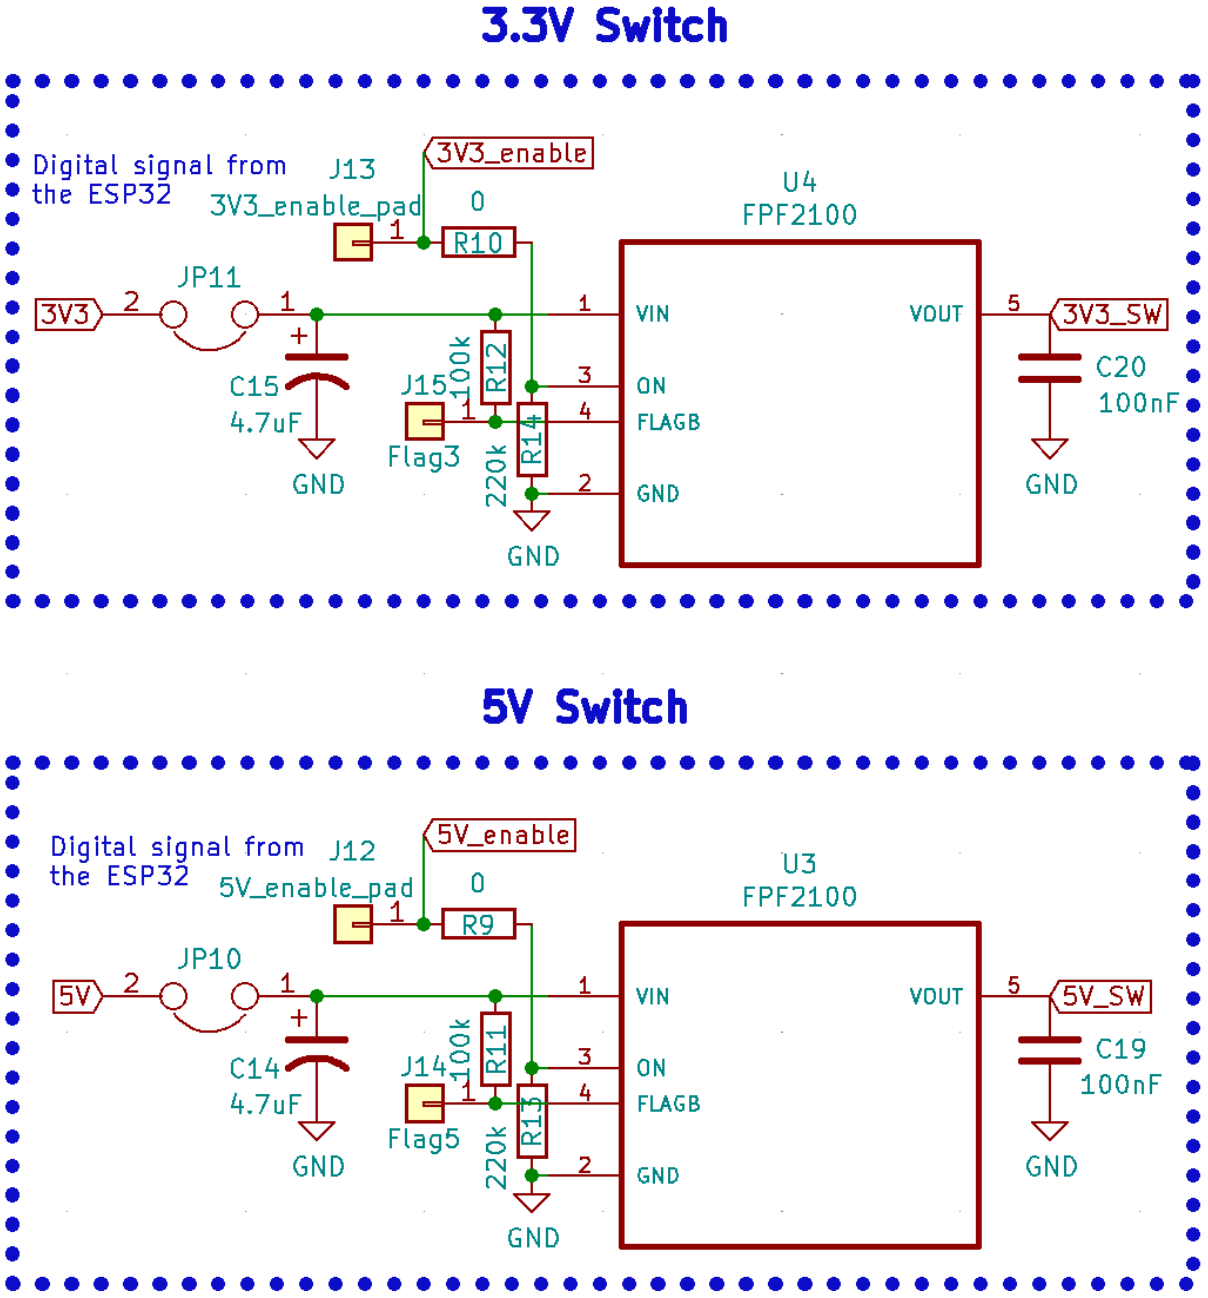
\includegraphics[width=0.7\linewidth]{Figures/cto_load_switch}
 	\caption{Circuito de encendido y apagado de las diferentes etapas de HW empleando un load switch FPF2100 \citep{fpf2100}.}
 	\label{fig:ctoloadswitch}
 \end{figure}\\
De esta manera las diferentes etapas de 3,3 V y 5 V se energizan unicamente cuando el MC pone en estado alto el pin \textit{ON} a la entrada del LS.\\
 
\subsection{Transformador de Intensidad}
Teniendo en cuenta que el comisionamiento debe realizarse sobre redes ya existentes y operativas, no resulta práctico utilizar un TI de núcleo sólido. Un TI de tipo nucleo partido como el presentado en la figura del ti  permite sortear el problema de interrumpir el cable a monitorear para enhebrarlo por el primario facilitar notablemente su comisionamiento o remoción.\\
\begin{figure}[h!]
	\centering
	\begin{subfigure}[b]{0.4\textwidth}
		\centering
		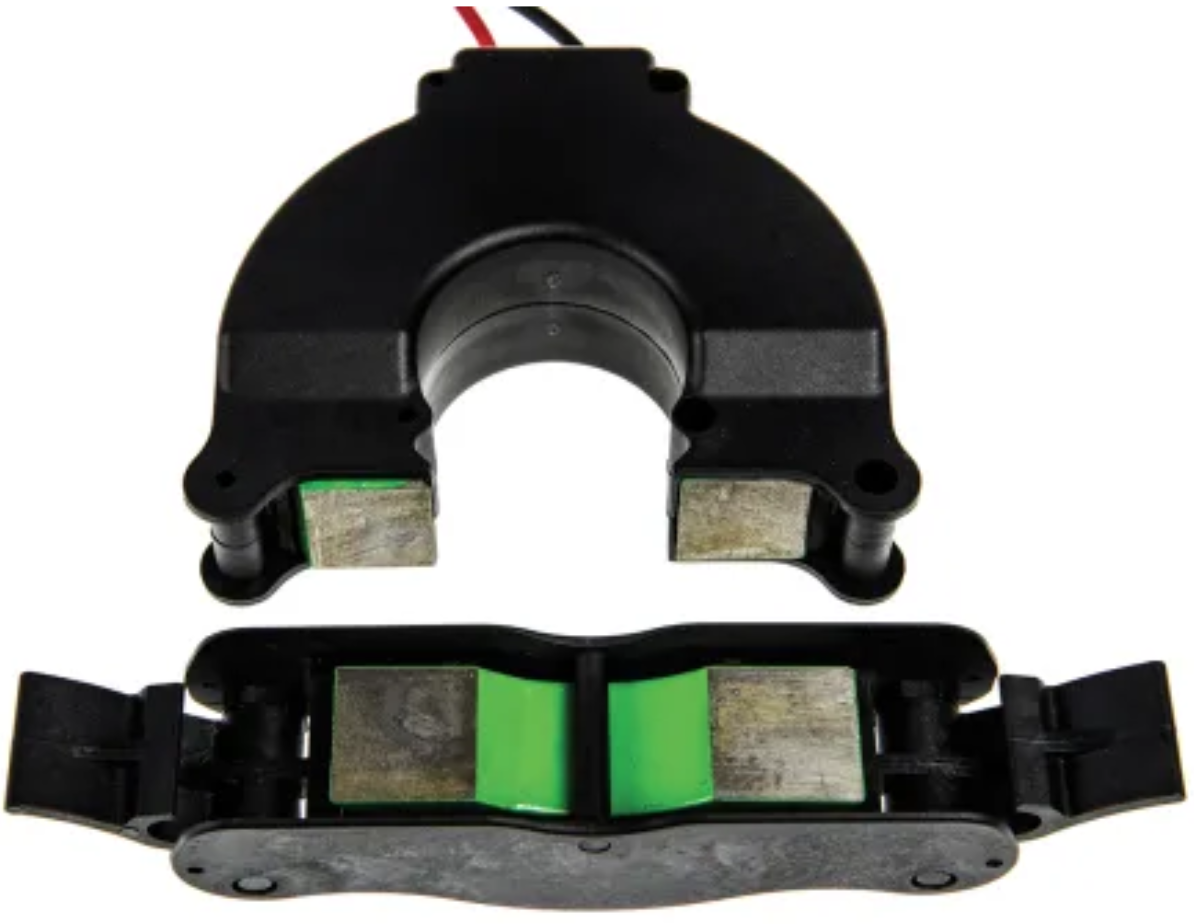
\includegraphics[width=.7\textwidth]{./Figures/ti_abierto}
		\caption{}
		\label{fig:ti_abierto}
	\end{subfigure}
	\centering
	\begin{subfigure}[b]{0.4\textwidth}
		\centering
		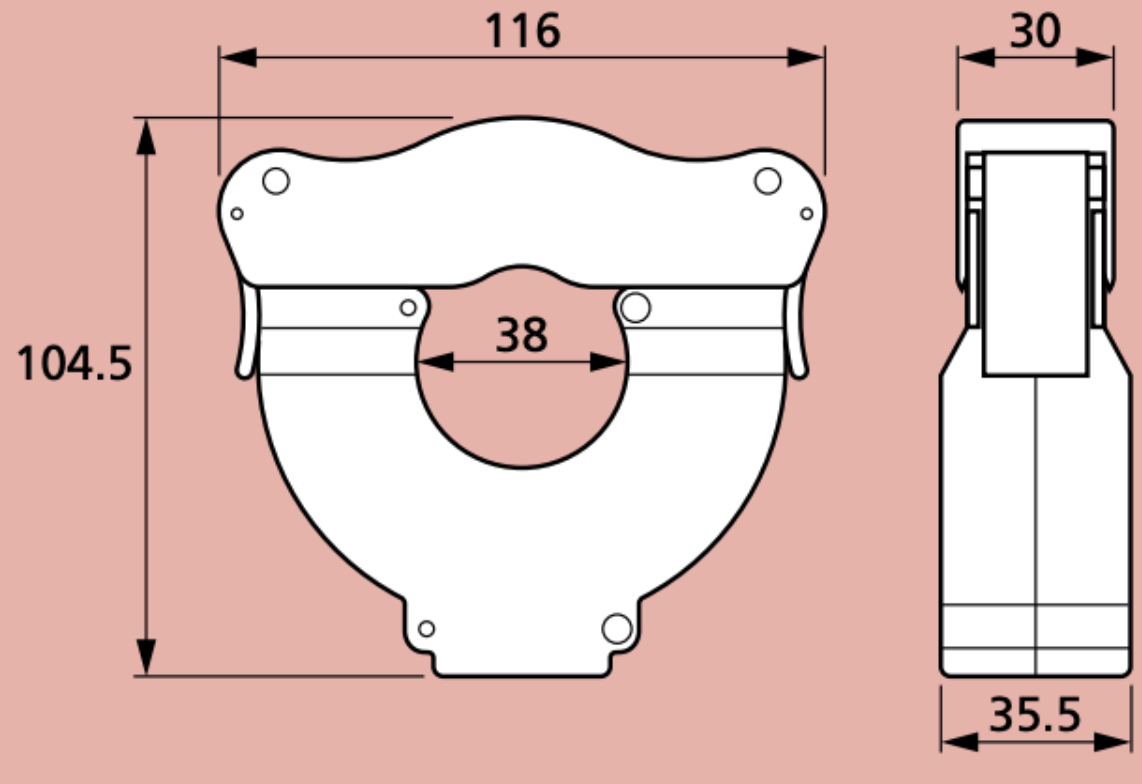
\includegraphics[width=.7\textwidth]{./Figures/ti_dimensiones}
		\caption{}
		\label{fig:ti_dimensiones}
	\end{subfigure}
	\caption{TI de tipo nucleo partido y sus dimenensiones. Imágenes tomadas de \citep{ct_hobut}}
	\label{fig:ti_mosaico}
\end{figure}\\
En base al requerimiento de corriente mínima admisible en circuito primario del TI, se eligió uno fabricado por la empresa Howard Butler Ltd modelo CTSCM40-200/5 y sus características se presentan en la \ref{tabla_caracteristicas_ti}.\\ 

\begin{table}
	\centering
	\caption{Características del CTSCM40-200/5 \citep{ct_hobut}}
	\begin{tabular}{lc} 
		\hline
		\multicolumn{1}{c}{Parametro}                                                       & \begin{tabular}[c]{@{}c@{}}Valor\\maximo~\end{tabular}  \\ 
		\hline
		Burden (VA)                                                                         & 2,5                                                     \\
		\begin{tabular}[c]{@{}l@{}}Corriente sobre el\\circuito primario (A)\end{tabular}   & 200                                                     \\
		\begin{tabular}[c]{@{}l@{}}Corriente sobre~el\\circuito secundario (A)\end{tabular} & 5                                                       \\
		\begin{tabular}[c]{@{}l@{}}Relacion de \\transformacion (N)\end{tabular}            & 40                                                      \\
		\begin{tabular}[c]{@{}l@{}}Rango de~\\frecuencia (Hz)\end{tabular}                  & 50 - 60                                                 \\
		Clase                                                                               & 1                                                       \\
		\hline
	\end{tabular}\label{tabla_caracteristicas_ti}
\end{table}

\subsection{Circuito de medición de valor RMS de corriente y acondicionamiento de señal}
Para medir corriente mediante un TI, es primero necesario convertir la intensidad en una señal de tensión representativa y partir de esta ahí calcular su valor RMS. Un resistor shunt de 0,1 Ohms con encapsulado TO-220-2 fue adoptado para convertir la corriente del secundario del TI en una señal de tensión apta para realizar su medicion RMS.\\
En el mercado existen circuitos integrados (CI) dedicados a cumplir esta tarea, estos funcionan generalmente otorgando una tension DC a la salida proporcional al valor RMS de la tension a la entrada. Una tabla comparativa resaltando el ancho de banda, la tensión pico a pico máxima admitida a sus entradas y tensión de operación de los posibles candidatos a utilizar en este proyecto se elaboró en la tabla \ref{tabla_chip_rms}\\
\begin{table}[h]
	\centering
	\caption{Tabla comparativa de chips aptos para medicion RMS}
	\begin{tabular}{cccc} 
		\hline
		Modelo                                & \begin{tabular}[c]{@{}c@{}}Ancho de Banda\\(BW)\end{tabular} & \begin{tabular}[c]{@{}c@{}}Vpp\\(max)\end{tabular} & \begin{tabular}[c]{@{}c@{}}Tension de\\operacion (max)\end{tabular}  \\ 
		\hline
		AD636 \citep{ad636}                                & 1,5 MHz                                                      & 283 mV                                             & 5 V                                                                  \\
		\textcolor[rgb]{0.2,0.2,0.2}{LH0091}\citep{lh0091}  & 2 MHz                                                        & +/- 15 V                                           & 22 V                                                                 \\
		\textcolor[rgb]{0.2,0.2,0.2}{LTC1966}\citep{ltc1966} & 800 kHz                                                      & +/- 1 V                                            & 5,5 V                                                                \\
		\hline
	\end{tabular}\label{tabla_chip_rms}
\end{table}
Por disponibilidad del autor al momento del ensayo se eligió el LTC1966 de la firma Linear Technologies.\\
El CI posee dos entradas \textit{IN1} e \textit{IN2} que se conectan a la señal tensión generada en bornes del shunt representado por \textit{R6} en el esquemático Figura RMS. A su salida \textit{VOUT}, otorga una tensión DC proporcional al valor RMS de la señal senoidal inyectada entre \textit{IN1} e \textit{IN2}.\\
Siend el valor máximo de un semiciclo de una onda senoidal en la entrada de 500 mV, el valor eficaz de esa señal de entrada y esperado a la salida del IC es
\begin{equation}
	Vrms=\frac{Vmax}{\sqrt{2}}=\frac{500}{\sqrt{2}}= 353,55 mV
\end{equation}
Los capacitores \textit{C10} y \textit{C12} se encargan de realizar el promedio y filtrar el posible ruido de alta frecuencia.\\
\textit{C9} y \textit{C11} filtran la tensión de alimentación que energiza al CI.\\
% TODO: \usepackage{graphicx} required
\begin{figure}[h!]
	\centering
	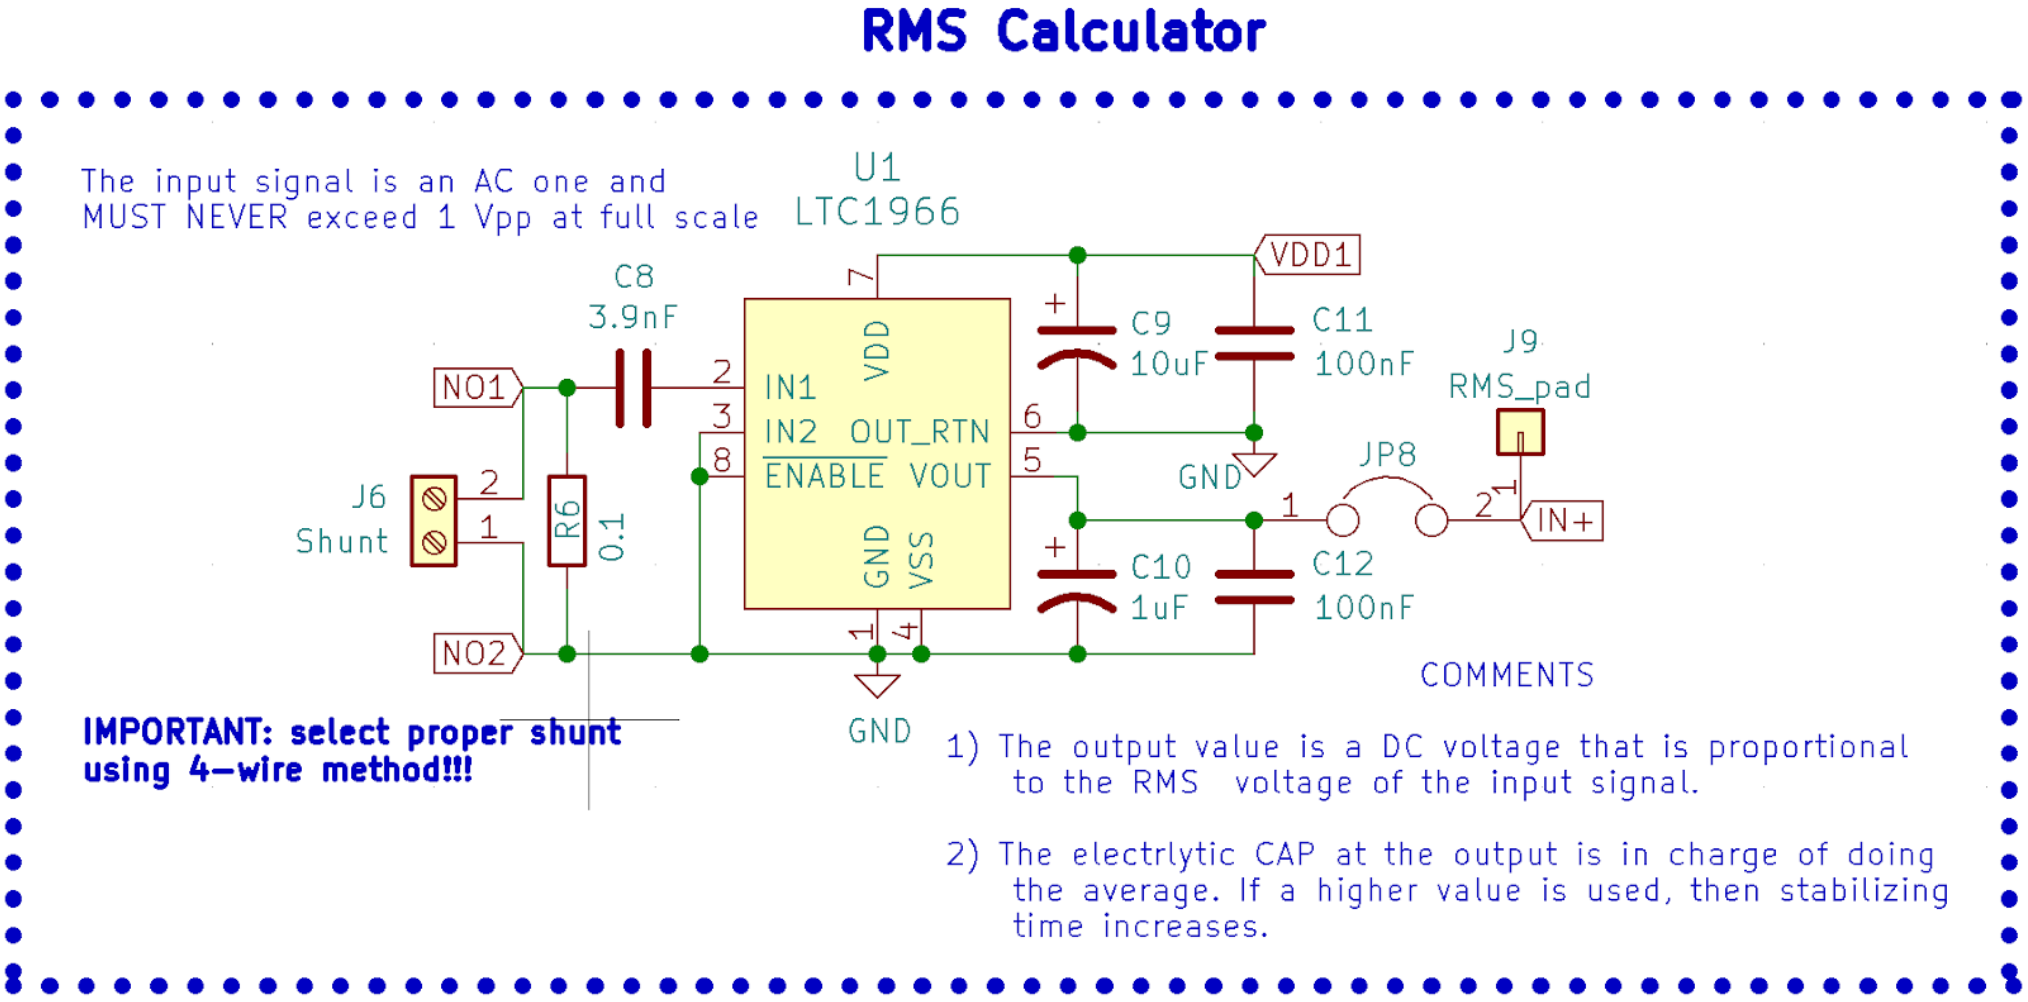
\includegraphics[width=0.7\linewidth]{Figures/cto_medidor_rms}
	\caption{Circuito medidor de valor RMS implementado usando el LTC1966.}
	\label{fig:ctomedidorrms}
\end{figure}
Dado que las mediciones a realizar se harán en líneas de distribución que operen a 50 Hz o 60 Hz, se ajustó la etapa de filtrado de la señal de entrada. Adoptada una impedancia de entrada de 8 Megaohms entre los pines IN1 e IN2 el capacitor C8 en serie forma un filtro pasa alto (HPF).\\
La frecuencia de corte (fc) adoptada por el autor para este HPF es de 5 Hz, por lo tanto
\begin{equation}
	fc = \frac{1}{2.\pi.R.C}\rightarrow\frac{1}{2.\pi.R.fc}\\
\end{equation}
\begin{equation}
	C=\frac{1}{2.\pi.8x10^6.5}=3,978x10^{-9} F
\end{equation}
El valor comercial más próximo adoptado para \textit{C8} fue entonces 3,9 nanofaradios.\\
Antes de conectar la señal de salida del LTC1966 es necesario amplificarla de modo que el fondo de escala de la medición tenga como máximo la misma tensión de alimentación que el ADC (3,3 V).\\
El circuito de la figura \ref{fig:ctoopamp}, utiliza un amplificador operacional MCP6001U \citep{mcp6001} en configuración amplificador no inversor. La ganancia de amplificacion \textit{A} del arreglo esta definida por
\begin{equation}
	A=\frac{R7+Pot1+R8}{R7}
\end{equation}

% TODO: \usepackage{graphicx} required
\begin{figure}[h!]
	\centering
	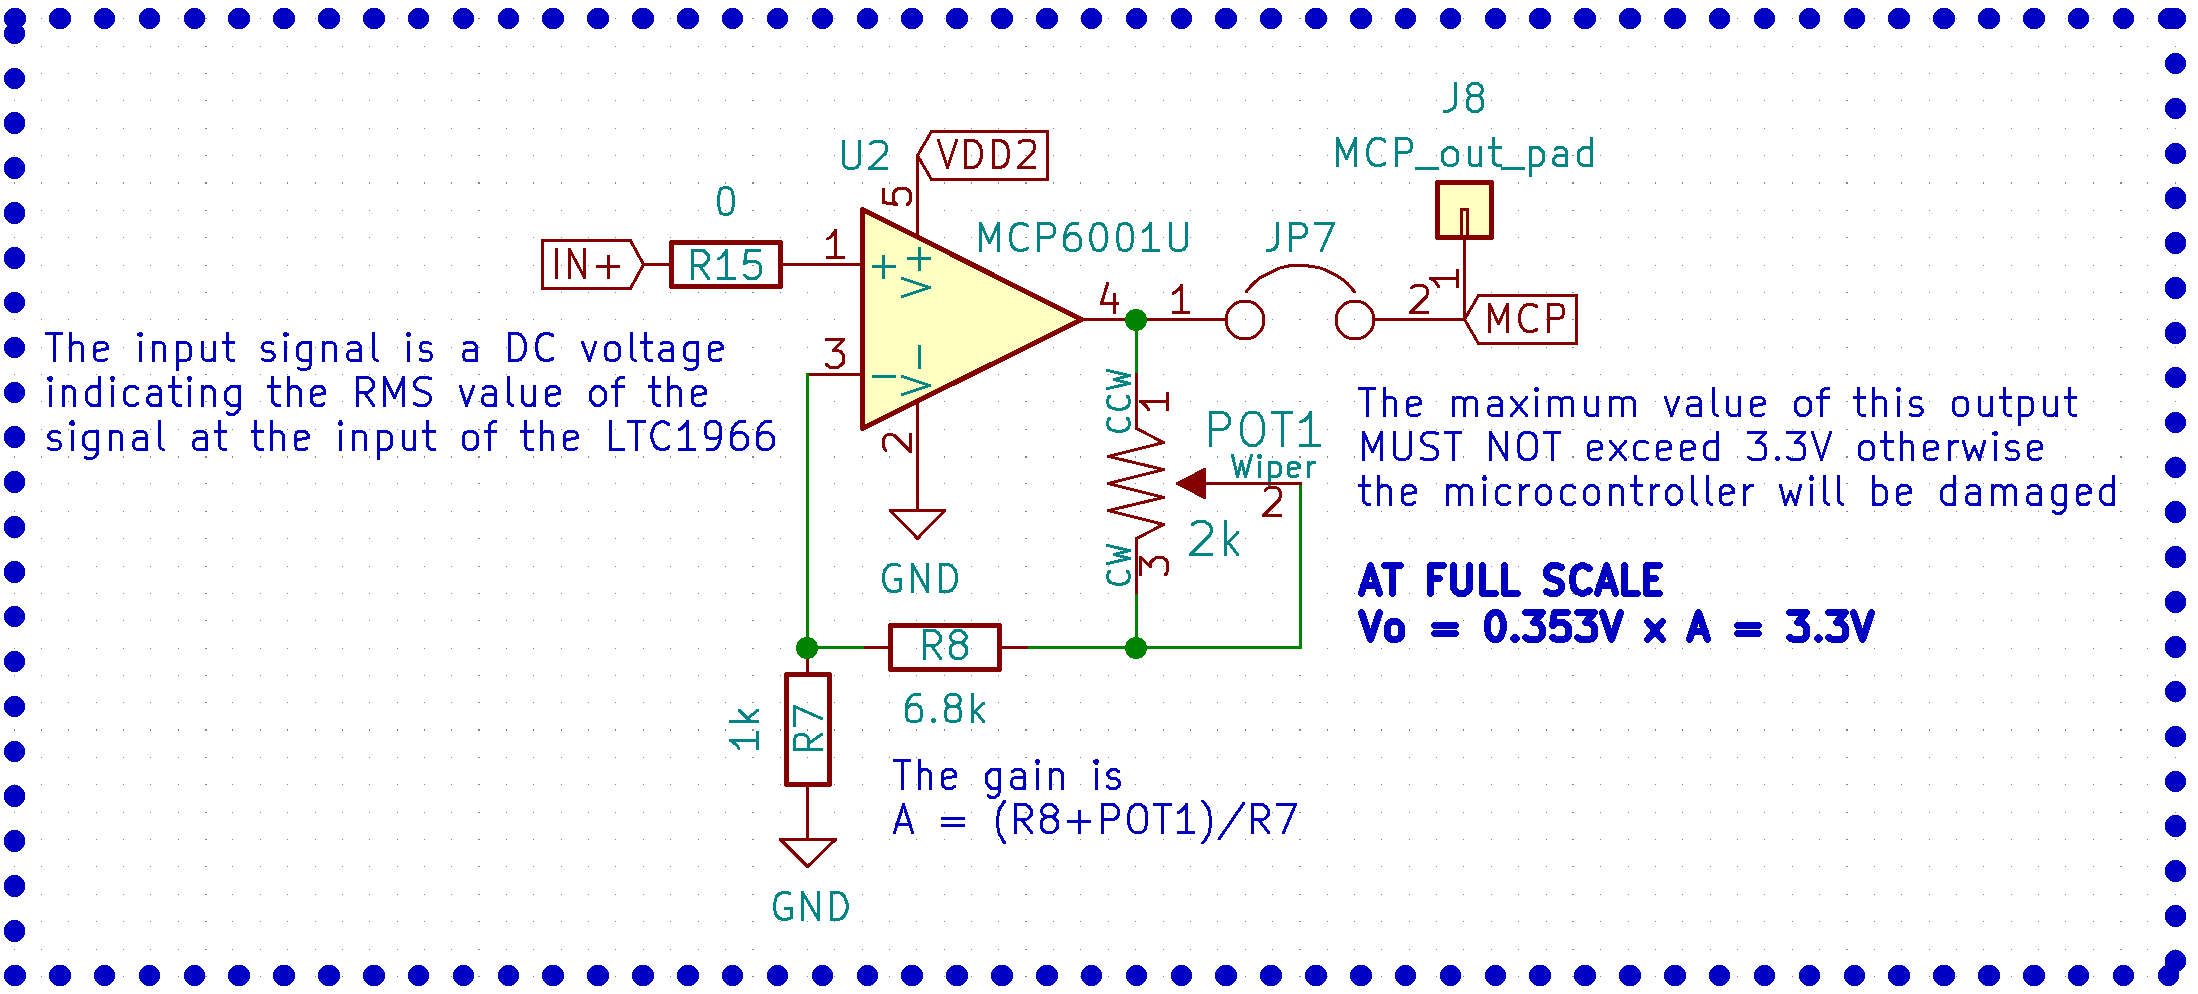
\includegraphics[width=0.7\linewidth]{Figures/cto_op_amp}
	\caption{Circuito amplificador de la senal de salida del LTC1966.}
	\label{fig:ctoopamp}
\end{figure}
Calibrada la ganacia del amplificador mediante una tension constante a la entrada \textit{IN+} y el potenciometro \textit{POT1}, la salida se encuentra lista para ser conectada a la entrada \textit{AIN0} del ADC.\\

\subsection{Monitoreo de tensión en bornes del acumulador}
La tensión máxima a la que puede llegar el acumulador de la figura \ref{fig:imagensupercap} es 5V, este valor de tensión es mayor que el máximo admitido por las entradas del ADC. Para obtener una senal de tension apta y equivalente a la tension en bornes del acumulador, es necesario atenuar la tension maxima a medir a una tension de 3,3V o menos.\\
El divisor resistivo formado por \textit{R4} y \textit{R5} implementado en el circuito de la Figura divisor resistivo SC, es una solucion efectiva para atenuar una senal de tension DC. De esta manera un valor de 5V en bornes del acumulador, representaria como maximo 2,5V a la entrada del ADC.\\
% TODO: \usepackage{graphicx} required
\begin{figure}[h!]
	\centering
	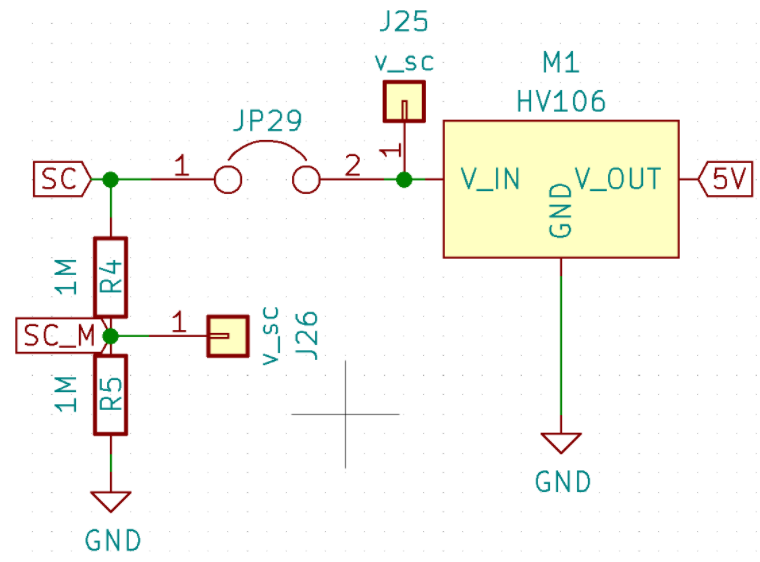
\includegraphics[width=0.7\linewidth]{Figures/cto_divisor_resistivo}
	\caption{Divisor resistivo utilizado para medir la tension en bornes del SC.}
	\label{fig:ctodivisorresistivo}
\end{figure}



\section{Firmware implementado}
\label{seccion_firmware}

\section{Servicios de Backend}
\label{seccion_bes}

\section{Integraci\'{o}n de la red LoRaWAN}

\section{Base de Datos}

\section{GUI basada en Grafana}

